% !TEX root = ../main.tex

\section{Area Between Two Curves}

\begin{myframe}[arc=10pt,auto outer arc]
Area between two curves $y=f(x)$ (upper function) and $y=g(x)$ (lower function) on the interval $[a, b]$ is given by
\[
A = \int_a^b \left(f(x) - g(x)\right) \, dx
\]
\end{myframe}

\problemans%
{Find the area of the region\\
bounded above by $y = x + 6$,\\
bounded below by $y=x^2$, and \\
bounded of the sides by the lines $x=0$ and $x=2$.}
{$\frac{34}{3}$}%

\problemans%
{Find the area of the region\\
that is enclosed between the curves\\
$y=x^2$ and $y=x+6$.}%
{$\displaystyle \frac{125}{6}$}%

\newpage

\problemans%
{Find the area of the region\\
that is enclosed between the curves\\
$x=y^2$ and $y=x-2$.
}%
{$\displaystyle \frac{9}{2}$}%

\makenewpage
\begin{myframe}[arc=10pt,auto outer arc]
Area between two curves $x=f(y)$ (right function) and $x=g(y)$ (left function) on the interval $[c, d]$ is given by
\[
A = \int_a^b \left(f(y) - g(y)\right) \, dy
\]
\end{myframe}

\problemans%
{Find the area of the region\\
that is enclosed between the curves\\
$x=y^2$ and $y=x-2$.
}%
{$\frac{9}{2}$}%

%\problemans%
%{Find the area of the region\\
%that is enclosed between the curves\\
%$x=y^2$ and $y=x-2$.
%}%
%{$\frac{9}{2}$}%

\makenewpage

\begin{myframe}[arc=10pt,auto outer arc]
	\noindent Area between a curve and the $x$-axis.
	
	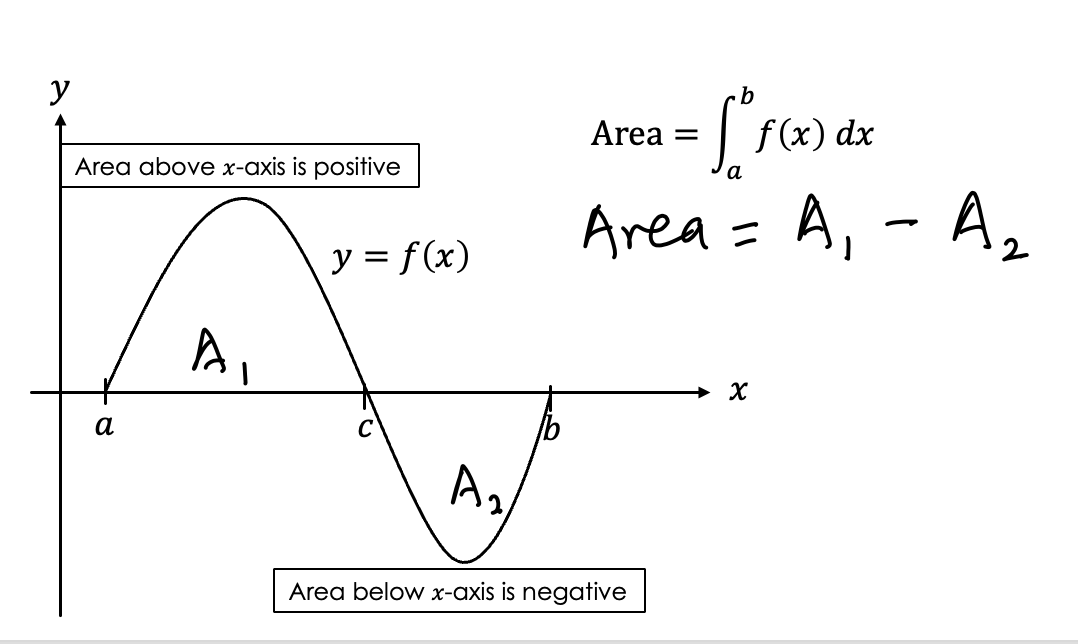
\includegraphics[width=0.7\linewidth]{chapter5/area}
\end{myframe}


\noindent Find the area under the curve $y=\cos{(x)}$ over the following intervals:

\pairofprobsans%
{$\displaystyle \left[0, \frac{\pi}{2}\right]$}{$1$}%
{$\displaystyle \left[\frac{\pi}{2}, \pi \right]$}{1}%

\problemans%
{$\displaystyle \left[0, \pi\right]$}{$$2}%

%%%% GUIDES
\qrfigure{chapter5/qr/Area-Between-Two-Curves}{Scan for guides}





